\documentclass[10pt]{article}

\usepackage{amsfonts, amsthm, fullpage, tikz}

\newcommand{\card}[1]{\left| #1 \right|}
\newcommand{\nat}{\mathbb{N}}
\newcommand{\ints}{\mathbb{Z}}
\newcommand{\reals}{\mathbb{R}}
\newcommand{\chtitle}[1]{\noindent \vspace{5mm}\textbf{Chapter #1}\vspace{3mm}}
\newcommand{\images}{/home/gparker/classes/341/images}

\begin{document}
\begin{center}
\textbf{
CS 341 Automata Theory \\
Elaine Rich \\
Homework 3 \\
Due Tuesday, Jan. 31}
\end{center}
This assignment covers Sections 5.1 -- 5.6. \\

\begin{enumerate}
\addtocounter{enumi}{1}
% ---
% 2
% ---

\item
Show a DFSM to accept each of the following languages:
\begin{enumerate}

\addtocounter{enumii}{1}
% b
\item
$\{w \in \{a, b\}^* : w$ does not end in $ba\}$.


% c
\item
$\{w \in \{0, 1\}^* : 2$ corresponds to the binary encoding, without leading $0$'s, of natural numbers that are evenly divisible by $4\}$.

% d
\item
$\{w \in \{0, 1\}^* : 2$ corresponds to the binary encoding, without leading $0$'s, of natural numbers that are powers of $4\}$.

\addtocounter{enumii}{2}
% g
\item
$\{w \in \{0, 1\}^* : w$ does not have $001$ as a substring $\}.$

\addtocounter{enumii}{4}
% l
\item
The set of binary strings with at most one pair of consecutive $0$'s and at most one pair of consecutive $1$'s.
\end{enumerate}

% ---
% 3
% ---

\item
Consider the children's game Rock, Paper, Scissors.  We'll say that the first player to win two rounds wins the game.  Call the two players $A$ and $B$.
\begin{enumerate}

%a
\item
Define an alphabet $\Sigma$ and describe a technique for encoding Rock, Paper, Scissors games as strings over $\Sigma$. (Hint: each symbol in $\Sigma$ should correspond to an ordered pair that describes the simultaneous actions of $A$ and $B$.)

%b
\item
Let $L_{RPS}$ be the language of Rock, Paper, Scissors games, encoded as strings as described in part (a), that correspond to wins for player $A$.  Show a DFSM that accepts $L_{RPS}$.
\end{enumerate}

% ---
% 4
% ---

\item
If $M$ is a DFSM and $\epsilon \in L(M)$, what simple property must be true of $M$?

\pagebreak
% ---
% 5
% ---

\item
Consider the following NDFSM M: \\

\begin{center}
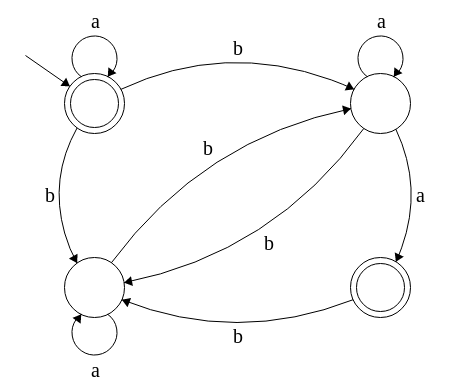
\includegraphics[scale=.5]{\images /hw3fsm5.png}
\end{center}

For each of the following strings $w$, determine whether $w \in L(M)$:
\begin{enumerate}
%a
\item
$aabbba$.

%b
\item
$bab$.

%c
\item
$baba$.
\end{enumerate}
% -
% 6
% -

\item
Show a possibly nondeterministic FSM to accept each of the following languages:
\begin{enumerate}

%a
\item
$\{a^nba^m : n, m \geq 0, n \equiv _3 m\}$.

%b
\item
$\{w \in \{o, 1\}^* : w$ contains both $101$ and $010$ as substrings\}.
\end{enumerate}


\pagebreak
\addtocounter{enumi}{2}
% ---
% 9
% ---

\item
Consider the following NDFSM. Use $ndfsmtodfsm$ to construct an equivilant DFSM.  Begin by showing the value of $eps(q)$ for each state $q$.

\begin{center}
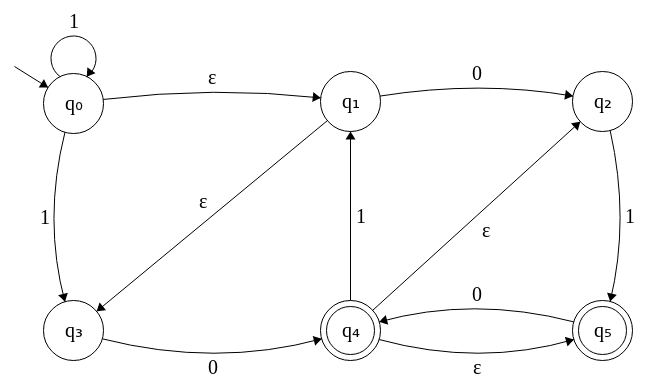
\includegraphics[scale=.5]{\images /hw3fsm9.png}
\end{center}
\end{enumerate}
\end{document}
